\documentclass[a4paper,10pt]{article}
\usepackage[utf8]{inputenc}
\usepackage[italian]{babel}
\usepackage[T1]{fontenc}
\usepackage{graphicx}
\usepackage{amsmath}
\usepackage{amssymb}
\usepackage{amsthm}
\usepackage{booktabs}
\usepackage{caption}
\usepackage{geometry}
%\usepackage{hyperref}
\usepackage{makeidx}
\usepackage{microtype}
\usepackage{subfig}
\usepackage{tabularx}
\usepackage{url}
\usepackage{varioref}
\usepackage{xcolor}
\usepackage{multicol}
\usepackage{mathtools}
\usepackage{booktabs}
\usepackage{multirow}
\usepackage{gensymb}
%\graphicspath{ {images/} }
\usepackage{float}
\usepackage{mathcomp}
\usepackage{placeins}
\usepackage{textcomp}
%%%%%%%%%%%%%%%%%%%%%%%%%%%%%%%%%%%%%%%%%%%%%%%%%%%
\makeindex
\begin{document}
\title{\textsc{Conducibilità termica}}
\author{Gabriele Di Ubaldo,\\ Andrea Torosantucci}
\date{12 Maggio 2016}
\maketitle
\begin{center}
\textit{\textbf{Univesrità di Pisa, Dipartimento di Fisica, \\ Laboratorio didattico del primo anno.}} \\
\end{center}
\begin{figure}[H]
 \centering 
 \includegraphics[width=2cm]{/home/zerch/Documents/UNIPI/Fisica1/images/unipi.jpg}
\end{figure} 
\tableofcontents
%%%%%%%%%%%%%%%%%%%%%%%%%%%%%%%%%%%%%%%%%%%%%%%%%%%%%%%%%%%%%%%%%%%%%%%%%%%%%%%%%%%%%%%%%%%%%%%%%%%%%%%%%%%%%%%%%%%%%%%%%%%%%%%%%%%%%%%%%%%%%%%%%%
\section{Obiettivo esperimento}
Avendo a disposizione due sbarre di diverso materiale riscaldate e raffreddate alle estremità contemporaneamente e potendo misurare tramite dei fori che variano in funzione della distanza,
lo scopo dell'esperienza è quello di misurare la condicibilità termica dei due materiali.
\subsection{Teoria e leggi}
La quantità di calore trasmessa per unità di tempo:
\begin{equation}
 W=\frac{dQ}{dt}
\end{equation}
Chiamato anche flusso di calore, questo all'equilbrio termico è costante. Chiamando S la sezione della sbarra, T la temperatura nei vari punti e d la distanza, la fomrula specifica diviene:
\begin{equation}
 W=-\lambda S\frac{\Delta T}{\Delta d}
\end{equation}
Nella quale $\lambda$ è chiamata conducibilità termica del materiale. Ovviamente dato che il calre fluisce spontaneamente dall zone più calda alla zona più fredda, il segno è negativo.
\subsubsection{Descrizione fenomeno}
\begin{figure}[H]
 \centering
 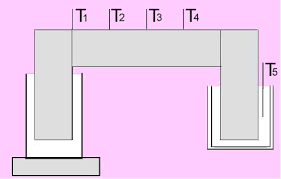
\includegraphics[width=8cm]{images.png}
 \caption{\textit{Immagine a scopo illustrativo}}
\end{figure}
\subsubsection{Apparato sperimentale}
\begin{itemize}
 \item Due barre cilindriche, di cui una rivestita di materiale isolante.
 \item Due termistori per la misura delle temperature.
 \item Calcolatore con programma di acquisizione (\textit{Plasduino}).
 \item Un alimentatore chiuso su due resistenze in parallelo.
 \item Un circuito ad acqua corrente.
 \item Calibro ventesimale (0.05mm)
\end{itemize}
%%%%%%%%%%%%%%%%%%%%%%%%%%%%%%%%%%%%%%%%%%%%%%%%%%%%%%%%%%%%%%%%%%%%%%%%%%%%%%%%%%%%%%%%%%%%%%%%%%%%
\section{Misure ed acquisizione dati}
Sistemato il voltaggio e l'amperaggio della corrente e azionato il flusso d'acqua, abbiamo incominciato ad eseguire delle misure tramite i termistori. Le misure ch abbiamo preso con i
termistori sono stae prese ponendo uno dei termistori all'estremità più calda e l'altro è stato inserito nei fori, cambiando posizione di volta in volta sino ad arrivare all'estremità
raffreddata dall'acqua corrente.\\
Il diametro interno ed esterno sono:$D_{esterno}=(2.51\pm0.05)cm$ e $D_{interno}=(0.7\pm0.1)cm$.\\
Il voltaggio é: $V=(10.1\pm0.1)V$ e l'amperaggio è: $I=(1.61\pm0.01)A$.\\
Inoltre i fori sono equispazioti di un $x_i=2.1\pm0.1cm$.
Per la vlautazoione di $\lambda$, abbiamo i valori tabulati per tre differenti materiali.
\begin{table}[H]
\centering
\caption{Valori tabulati}
\label{my-label}
\begin{tabular}{|l|l|l|}
\hline
Materiale & \multicolumn{2}{l|}{$\lambda$ {[}W/(m °C){]}} \\ \hline
Alluminio & \multicolumn{2}{l|}{$\sim$ 200}               \\ \hline
Rame      & \multicolumn{2}{l|}{$\sim$ 400}               \\ \hline
Ottone    & \multicolumn{2}{l|}{$\sim$ 110}               \\ \hline
\end{tabular}
\end{table}
\subsection{Misure}
Abbiamo preso rispettivamente 20 misure di temperatura, equivalenti ad ogni foro presente sulla sbarra.
In seguito durante la presa dati abbiamo lasciato i termistori per un tempo ragionevolmente lungo ($\approx 40 secondi$), affinchè il sistema andasse all'equilibrio.
La prima temperatura è stata presa facendo la media della misure e la seconda temperatura (quella misurata del secondo termistore che è stato spostato di volta in volta) è stata calcolata 
acìnch'essa facendo la media delle misure registrate.
Per la sbarra non isolata abbiamo ottenuto:
\begin{table}[H]
\centering
\caption{\textbf{Sbarra non isolata}}
\label{my-label}
\begin{tabular}{|l|l|}
\hline
\multicolumn{2}{|l|}{Temperature sbarra non isolate (°C)} \\ \hline
T1                         & 37.20                        \\ \hline
T2                         & 36.52                        \\ \hline
T3                         & 35.11                        \\ \hline
T4                         & 34.52                        \\ \hline
T5                         & 33.73                        \\ \hline
T6                         & 32.80                        \\ \hline
T7                         & 31.86                        \\ \hline
T8                         & 30.91                        \\ \hline
T9                         & 30.54                        \\ \hline
T10                        & 29.67                        \\ \hline
T11                        & 28.99                        \\ \hline
T12                        & 28.12                        \\ \hline
T13                        & 27.60                        \\ \hline
T14                        & 26.69                        \\ \hline
T15                        & 26.47                        \\ \hline
T16                        & 25.63                        \\ \hline
T17                        & 24.91                        \\ \hline
T18                        & 23.79                        \\ \hline
T19                        & 23.76                        \\ \hline
T20                        & 22.74                        \\ \hline
\end{tabular}
\end{table}
Per la sbarra isolata abbiamo ottenuto:
\begin{table}[H]
\centering
\caption{\textbf{Sbarra isolata}}
\label{my-label}
\begin{tabular}{|l|l|}
\hline
\multicolumn{2}{|l|}{Temperature sbarra non isolate (°C)} \\ \hline
T1                         & 57.35                        \\ \hline
T2                         & 54.72                        \\ \hline
T3                         & 54.33                        \\ \hline
T4                         & 51.74                        \\ \hline
T5                         & 49.49                        \\ \hline
T6                         & 48.23                        \\ \hline
T7                         & 46.03                        \\ \hline
T8                         & 44.76                        \\ \hline
T9                         & 42.38                        \\ \hline
T10                        & 41.01                        \\ \hline
T11                        & 38.48                        \\ \hline
T12                        & 37.19                        \\ \hline
T13                        & 35.30                        \\ \hline
T14                        & 33.79                        \\ \hline
T15                        & 32.13                        \\ \hline
T16                        & 30.42                        \\ \hline
T17                        & 29.11                        \\ \hline
T18                        & 27.21                        \\ \hline
T19                        & 25.33                        \\ \hline
T20                        & 23.43                        \\ \hline
\end{tabular}
\end{table}
\textbf{\large Come incertezze sulle misure di temperatura prendiamo un $\Delta T= 0.35$ \textcelsius}
\section{Analisi dati}
Prese le misure, possiaamo ricavare la sezione delle sbarre e la potenza dissipata.
\begin{equation}
 W=\frac{VI}{2}
\end{equation}
Questa è valida per resistenze in parallelo.
Invece per la sezione possiamo usare:
\begin{equation}
 S=\frac{\pi(D_{esterno}^2-D_{interno}^2)}{4}
\end{equation}
In questo modo otteniamo:$W=(8.13\pm0.13)W$, $S=(4.5\pm0.3)cm^2$.
\subsection{Propagazione degli errori}
L'errore è stato già calcolato precendentemente nella varie formule, dunque nella seguente sezione non abbiamo nulla di rilevante da osservare.
\section{Fit grafico ed elaborazione dati}
Presi i dati andremo a tracciare tramite GNUplot (\textit{che utilizza l'algoritmo di Marquardt-Levenberg}) a tracciare il grafico della temperatura in funzione della distanza;
possiamo prevedere che dato il flusso spontaneo di calore, la retta avrà coefficiente angolare negativo che sarà la stima di $-\frac{W}{\lambda S}$ dalla quale ricaveremo la conducibilità termica.
\subsection{Fit grafico}
Qui riportiamo il seguente fit:
\begin{figure}[H]
 \centering
 \caption{Sbarra non isolata}
 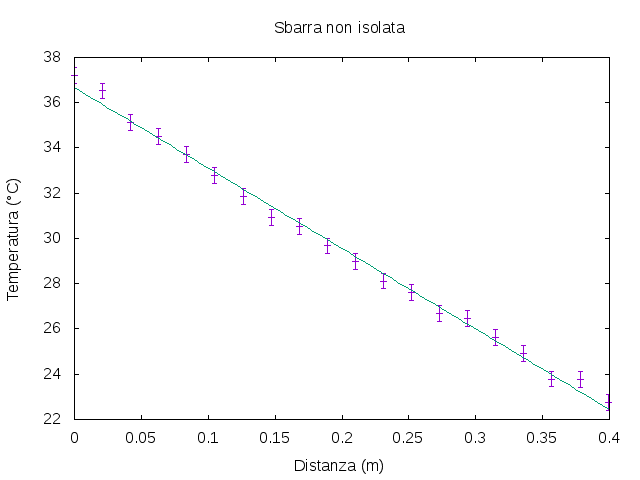
\includegraphics[width=11cm]{Non isolata.png}
\end{figure}
Sulla sbarra isolata le misure sono più imprecise, tuttavia si riesce in ogni caso a stimare $\lambda$.
Qui riportiamo l'ulteriore grafico:
\begin{figure}[H]
 \centering
 \caption{Sbarra isolata}
 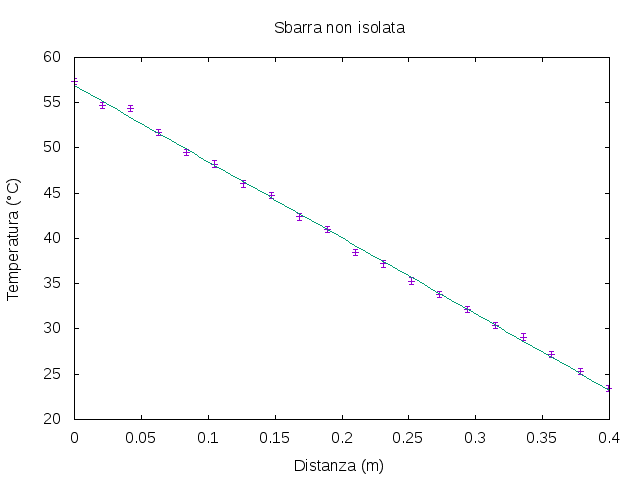
\includegraphics[width=11cm]{Isolata.png}
\end{figure}
Ora tracciato il fit ed avendo stimato tramite esso i valori della retta, possiamo stimare $\lambda$.
\subsection{Elabborazione dati}
La funzione utilizzata per fare il fit è del tipo: y=Ax+B. Teoricamente questa è la funzione di fit della funzione ricavata prima dalla formula del flusso di calore, ossia:
\begin{equation}
 T_i=T_0-\frac{W}{\lambda S}x_i
\end{equation}
Infatti dal fit stimiamo A e B che equivalgono a $T_0$ e $-\frac{W}{\lambda S}$.\\
Innanzitutto come possiamo notare nei fit abbaimo B e dunque $T_0$; nel fit della sbarra non isolata otteniamo $T_0=36.67\pm0.14$ contro il valore misurato $T_0=37.20\pm0.35$,
possiamo calcolare la discrepanza tra queste misure.\\
Vedendo che questa è minore dell'errore propagato sulla differenza possiamo dire che il modella ripsetta verifica i dati sperimentali.
\begin{equation}
 Discrepanza=\left | T_{stimato}-T_{misurato} \right |
\end{equation}
\begin{equation}
 \Delta Discrepanza=\delta T_{stimato} + \delta T_{misurato}
\end{equation}
Ora se la $Discrepanza\ll\Delta Discrepanza$ allora il modello è verificato.\\
Infatti: $\Delta Discrepanza= 0.49$ e $Discrepanza=0.53$.\\
Dato che non è molto minore, possiamo affermare che la discrpanza non è significativa.\\
Lo stesso ragionamento operato sulla sbarra isolata permette di ottenere:\\
$\Delta Discrepanza=0.52$ e $Discrepanza=0.44$.\\
Anche in questo caso in prima approssimazione, la discrepanza non è significativa.
Ora calcoliamo il coefficiente angolare, per il primo grafico abbiamo ottenuto $A=-35.56\pm0.60$, sapendo che $A=-\frac{W}{\lambda S}$ otteniamo che:\\
\begin{displaymath}
 \lambda=\frac{W}{AS}
\end{displaymath}
propagando l'errore,
\begin{displaymath}
 \Delta \lambda=\left | \frac{\partial\lambda}{\partial W} \right | \Delta W + \left | \frac{\partial\lambda}{\partial S} \right | \Delta S +  \left | \frac{\partial\lambda}{\partial A} \right | \Delta A
\end{displaymath}
In questo modo la conducibilità termica per la sbarra non isolata è: $\lambda=(508\pm83)$\textcelsius C, che bsandoci sulle conducibilità tabulate, entro la barra d'errore possiamo dire concide 
approssimativamente con il rame.
Allo stesso modo per la barra isolata otteniamo $A=(-86.17\pm0.75)$ dunqueotteniamo che:  $\lambda=(210\pm11)$\textcelsius C, alla stessa maniera, guardando le conducibilità tabulate, pppossiamo ricondurre la seconda
sbarra al materiale alluminio.
Infine il Test del $\chi^2$ in entrambi i grafci ha rilevato valori accettabili entro le convenzioi:
I gradi di libertà sono 18 e per la sbarra non isolata otteniamo un $\chi^2=15.66$, avendo questa probabilità:
\begin{displaymath}
 P(\chi^2\leq15.66)\approx38.4\%
\end{displaymath}
Per la secondo sbarra isolata otteniamo un $\chi^2=24.26$, avendo questa probabilità:
\begin{displaymath}
 P(\chi^2\leq24.26)\approx85.34\%
\end{displaymath}
In ultima analisi possiamo vedere il grafico dei residui per vedere se il modello rispetta la realà:
\begin{figure}[H]
 \centering
 \caption{Residui sbarra non isolata}
 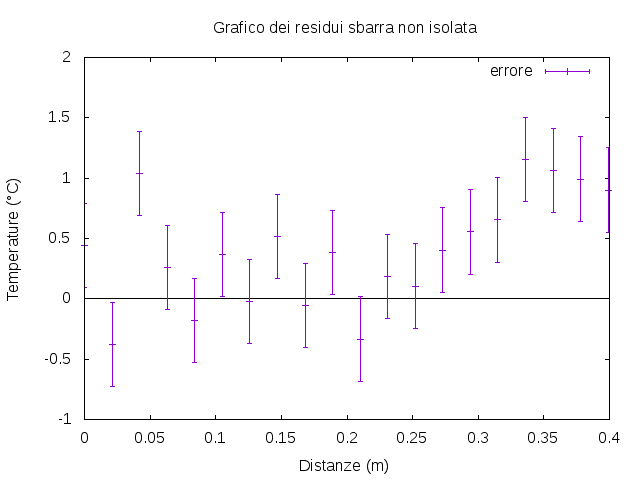
\includegraphics[width=11cm]{Residui non isolata.png}
\end{figure}
\begin{figure}[H]
 \centering
 \caption{Residui sbarra isolata}
 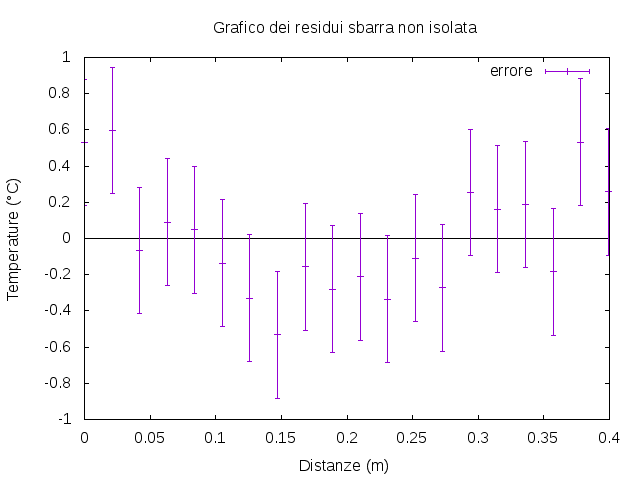
\includegraphics[width=11cm]{Residui isolata.png}
\end{figure}
Da queste possiamo rilevare una sottostima degli errori per la sbarra non isolata, tuttavia sembrano disporsi in maniera piuttosto casuale e questo vale anche per la seconda sbarra.
\section{Conlcusioni}
Possiamo concludere che alla luce di tutta la presa ed analisi dati, il nostro modello rispechia i dati misurati entro errori non significativi, grazie alla discrepanza valutata precendentemente e 
grazie al test del $\chi^2$ che ci ha indicato una buona probabilità di trovare un valore più basso reiterando le misure, questo ci indica una buona concordanza con il modello teroico e i dati sperimentali.
L'esperimento può dirsi concluso.
\end{document}
